\chapter{Introdução ao Python}\label{ch:1}

Python é uma poderosa linguagem de programação de propósito geral desenvolvida por Guido van Rossum\footnote{Quando começou a implementar o primeiro interpretador Python, Guido van Rossum também estava assistindo a série ``Flying Circus'' do famoso grupo de comédia Inglês ``Monty Python''. Van Rossum pensou que precisava de um nome que fosse curto, único e um pouco misterioso, então decidiu chamar a linguagem de Python} em 1989.  É classificada como uma linguagem de programação de alto nível na medida em que lida automaticamente com as operações mais fundamentais (como gerenciamento de memória) realizada no nível do processador (“código de máquina”). É considerado um nível superior linguagem do que, por exemplo, C++, por causa de sua sintaxe (que é próxima de linguagem natural, no caso o inglês) e rica variedade de estruturas de dados nativas, como listas, tuplas, conjuntos e dicionários (vamos discutir um pouco delas no Apêndice \ref{ap:1.1}). Na verdade o Python, como outras linguagens de alto nível, é um interpretador. Em uma linguagem interpretada como o Python, cada comando é analisado e convertido “ao longo do caminho”. Esse processo torna a linguagem interpretada significativamente mais lenta; mas a vantagem é que elas são mais simples para se programar ajustar e depurar porque você não tem para recompilar o programa após cada alteração.

O Python apresenta algumas vantagens:
\begin{enumerate}
    \item Sua sintaxe limpa e simples torna a escrita de programas Python rápida, simples e geralmente minimiza as chances para que os bugs se infiltrem.
    \item É gratuito – Python e suas bibliotecas  associadas são gratuitas e de código aberto, ao contrário de ofertas comerciais como Mathematica e MATLAB.
    \item Suporte multiplataforma: Python está disponível para todos os com-
computador, incluindo Windows, Unix, Linux e macOS.
    \item O Python possui uma grande biblioteca de módulos e pacotes que estendem sua funcionalidade. Isso é ferramentas já prontas que nos permitem realizar uma diversidade de operações complexas comuns como as de álgebra linear, derivação, integração, operações matemáticas simbólicas, construção de gŕaficos. Muitos deles estão disponíveis como parte da “Biblioteca Padrão” fornecida com o próprio Python. Outros, incluindo o NumPy, SciPy, Matplotlib (algumas dessas estão discutidas nos Apêndices) e bibliotecas pandas usadas em computação científica, podem ser baixadas gratuitamente.
    \item Python é relativamente fácil de aprender. A sintaxe e as expressões idiomáticas usadas para operações básicas são aplicados de forma consistente no uso mais avançado da linguagem. Mensagens de erro geralmente são avaliações significativas do que deu errado, e não os alertas genéricos de “travamentos” que podem ocorrer em linguagens compiladas de baixo nível.
    \item Python é flexível: muitas vezes é descrito como uma linguagem “multi-paradigma” que contém os melhores recursos dos paradigmas procedimentais, orientados a objetos e funcionais.
\end{enumerate}

É claro que o Python também possui algumas desvantagens:
\begin{enumerate}
    \item A velocidade de execução de um programa Python não é tão rápida linguagens de mais baixo nível como C++ e Fortran. Para aplicações numéricas pesadas, algumas bibliotecas como o NumPy e o SciPy minimizam essa perda de velocidade pois elas mesmas são códigos C++ escondidos sobre uma ``tradução'' para Python. 
    \item Para fornecer simplicidade a linguagem, o Python usa quantidade de memória maior. Isso pode ser uma desvantagem ao criar aplicações que demandem um uso otimizado de memória. Por essa razão e pela menor velocidade, o Python é pouco utilizado para aplicativos móveis e para servidores.
    \item Python é uma linguagem dita dinâmica. Com isso uma variável que em um dado momento do código é um número inteiro, em outro ponto do código pode ser tornar uma string (e.g. um texto). Isso se chama {\it Mutabilidade} e pode gerar alguns erros. Isso requer que códigos mais complexos sejam bastante testados.
\end{enumerate}

Em resumo, Python é uma linguagem de programação moderna e bem projetada, ao mesmo tempo fácil de aprender e muito poderosa. Ou seja embora seja simples o suficiente para permitir que estudantes sem experiência prévia em programação resolvam problemas já início da graduação, O Python também é poderoso o suficiente para ser usado para trabalho numérico em física. Na próxima seção, discutimos como instalar o Python em um sistema operacional Linux.

\section{Instalação}\label{sc:1.1}

Verifique se já tem o Python instalado, se você usa GNU/Linux, provavelmente já possui alguma versão do Python instalada por padrão. Para conferir, digite em um terminal:

\begin{lstlisting}[language=bash]
  $ which python3
\end{lstlisting}
O Python 3 é a versão atual do Python\footnote{O Python 2 foi descontinuado em 2020.}, por ser o futuro da linguagem e pelo fato de sua versão anterior estar em processo de descontinuação.
Caso o Python esteja instalado, o sistema vai retornar algo como
\begin{lstlisting}[language=bash]
  /usr/bin/python
\end{lstlisting}
Caso contrário, o sistema retornará algo do tipo
\begin{lstlisting}[language=bash]
  which: no python 
  in (/usr/local/sbin:/usr/local/bin:/usr/bin:/usr...)
\end{lstlisting}

Caso o Python não esteja instalado podemos instala-lo via um gerenciador de pacotes da distribuição do Linux instalada na máquina. Os gerenciadores de pacotes mais comuns são apt-get que funcionam em distribuições como o Debian, o Ubuntu e o Mint. Para instalar o Python usando o apt-get digite em um terminal:
\begin{lstlisting}[language=bash]
  $ sudo apt-get install python3
\end{lstlisting}
É comum que no desenvolvimento de projetos Python, precisemos instalar diversas bibliotecas para diferentes necessidades. Essas bibliotecas podem ser instaladas manualmente, mas o processo pode ser complicado. Para contornar esse problema, o Python possui uma ferramenta para gerenciamento de pacotes chamado PIP. Isso em geral não é necessário em distribuições Linux como Debian, Ubuntu e Mint. Para instalar o gerenciador de pacotes pip, digite em um terminal:

\begin{lstlisting}[language=bash]
  $ sudo apt-get install python3-pip
\end{lstlisting}
Caso sua distribuição utilize um gerenciador de pacotes diferente deste (ou você utilize Windows) {\it \bf não entre em pânico}, na internet há instruções passo a passo para instala-lo. 

Para ver a versão do Python que você tem instalado digite no terminal
\begin{lstlisting}[language=bash]
  $ python3 --version
\end{lstlisting}
Após a instalação você poderá usar o Python diretamente do terminal. Por exemplo, digite
\begin{lstlisting}[language=bash]
  $ python
  $ 6*7
  $ a=10**3
  $ print(a)
  $ quit()
\end{lstlisting}

É claro seria muito inconivente escrever um código diretamente no terminal. Precisamos agora instalar uma IDE (ambiente de desenvolvimento integra, do inglês {\it Integrated Development Environment}). Existem várias IDE para Python, durante o curso utilizaremos o Jupyter-Notebook. Para instala-la digite no terminal:

\begin{lstlisting}[language=bash]
  $ sudo apt-get install jupyter-notebook
\end{lstlisting}

Para iniciar o notebook digite no terminal o seguinte comando:
\begin{lstlisting}[language=bash]
  $ jupyter-notebook
\end{lstlisting}
O Jupyter Notebook deverá abrir em seu browser de internet.

\section{Primeiros Passos no Jupyter Notebook}

Quando o Jupyter Notebook abrir em seu navegador você verá o Dashboard do Jupyter Notebook, o qual irá exibir uma lista dos notebooks, arquivos e subdiretórios no diretório onde o servidor do notebook foi inicializado. Na maioria das vezes, você irá querer que o servidor do notebook inicie no diretório de nível mais alto que contenha os notebooks. Geralmente este será seu diretório home. A tela deve se parecer com a tela abaixo (Fig. \ref{fig:JN-Dashboard})
\begin{figure}[h!]
\centering
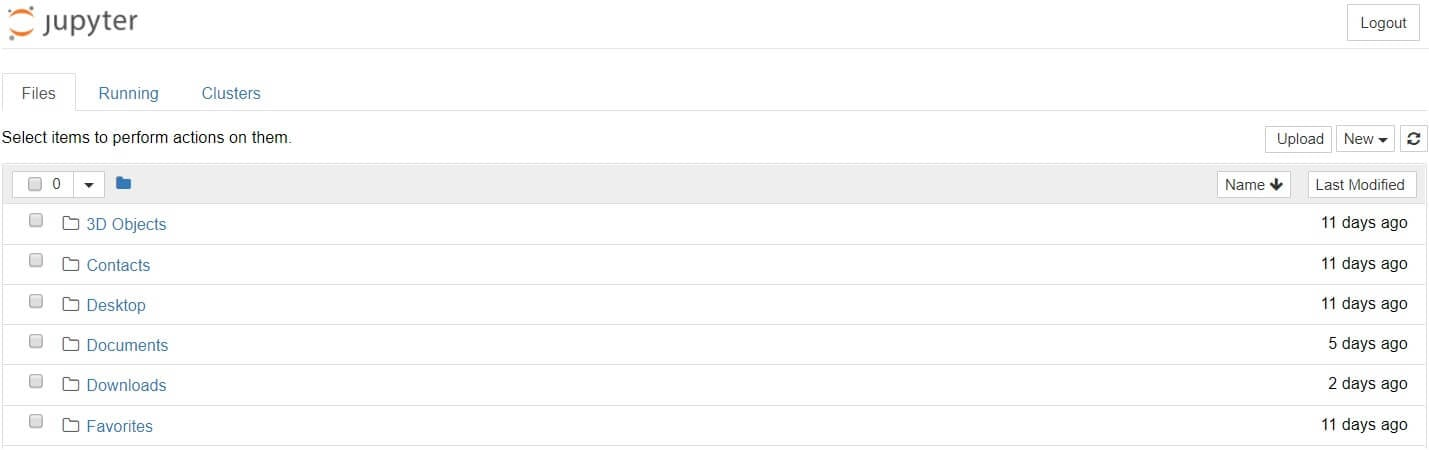
\includegraphics[scale=0.3]{Images/jupyter-dashboard.jpg}
\caption{Exemplo do Dashboard do Jupyter Notebook, a primeira tela que você deve ver quando abre o Jupyter.}\label{fig:JN-Dashboard}
\end{figure}
Isso ainda não é o que chamamos de um notebook, mas {\it \bf não entre em pânico}. O dashboard é o gerenciador de arquivos que seve para você selecionar, procurar e organizar seus notebooks. A interface é bastante simples de se entender. Vamos começar criando um diretório para guardarmos nossos projetos em Python. Para isso clique no menu {\tt New} no canto superior direito e selecione a opção {\tt Folder} (veja a Fig. \ref{fig:JN-NEW}.)
\begin{figure}[h!]
\centering
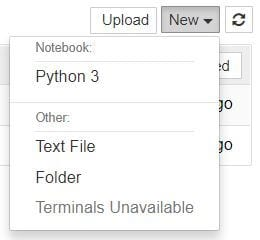
\includegraphics[scale=0.4]{Images/new-notebook-menu.jpg}
\caption{O menu {\tt New} permite abir um novo ({\tt Python 3}), criar um arquivo de texto ({\tt Text File}), Folder ({\tt Folder}) ou abrir um terminal ({\tt Termial}).}\label{fig:JN-NEW}
\end{figure}
O diretório é criado com o nome {\tt Untitled Folder} (i.e. dirétório sem título). Para renomear um folder ou arquivo, no dashboard, você deve marcar a caixa de seleção à esquerda do nome do folder ou arquivo e clicar na opção {\tt Rename}, que fica disponível na barra de menu após a caixa de seleção ser ativada (veja a Fig. \ref{fig:JN-Rename}.)
\begin{figure}[h!]
\centering
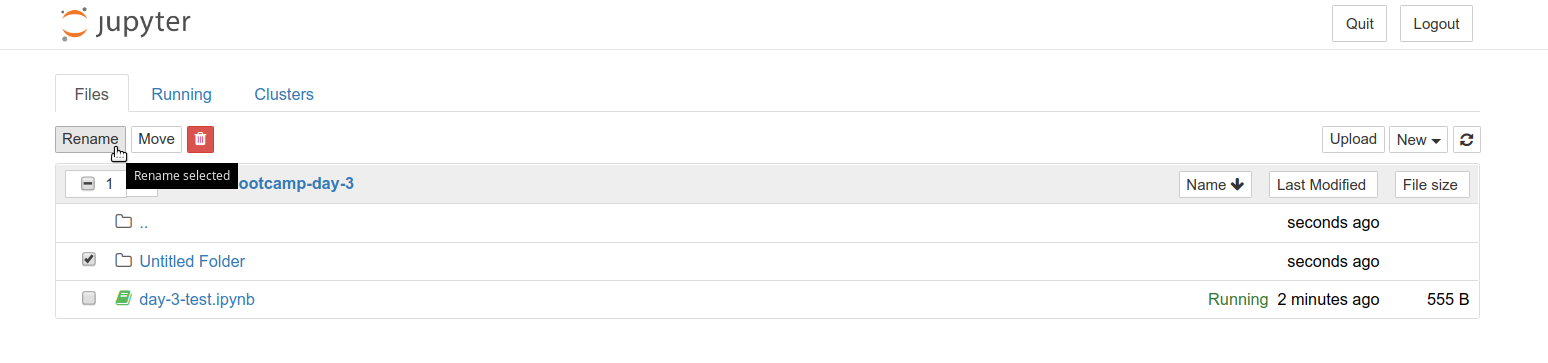
\includegraphics[scale=0.28]{Images/rename-folder.png}
\caption{Marcando a caixa de seleção de um arquivo ou folder você pode renomeá-lo ({\tt Rename}), mover sua localização na árvore de diretórios ({\tt Move}) ou deleta-lo (ícone da lixeira). }\label{fig:JN-Rename}
\end{figure}

Vamos agora criar um notebook, para isso selecione a opção {\tt Python 3} no menu {\tt New}. Uma tela como a abaixo deverá aparecer (veja a Fig. \ref{fig:JN-Notebook})
\begin{figure}[h!]
\centering
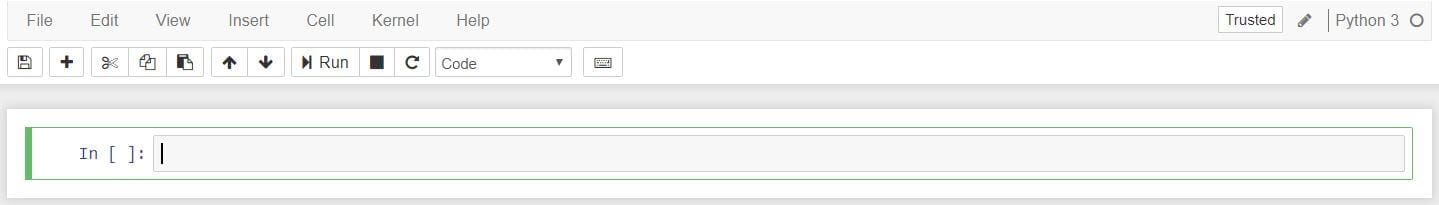
\includegraphics[scale=0.3]{Images/new-notebook.jpg}
\caption{Tela inicial de um notebook}\label{fig:JN-Notebook}
\end{figure}
No menu superior, você verá opções tradicionais como {\tt File}, {\tt Edit}, {\tt View}, {\tt Insert} e {\tt Help}, suas funções são intuitivas e você pode explora-las para conhecer suas funcionalidades. Nesse Menu aparecem dois termos importantes: {\tt Cell} (células) e {\tt Kernel} (núcleos).
\begin{itemize}
    \item {\bf Kernel:} é o nome dado pelo Jupyter Notebook a um “mecanismo computacional” que interpreta o código contido em um documento de notebook. Haverá um kernel para cada linguagem suportada pelo Jupyter Notebook. Basicamente, um kernel Python 3 conversa com o kernel do sistema operacional (no caso um kernel Linux) para executar os comandos.
    \item {\bf Cell:} é um bloco para o texto a ser exibido no notebook ou código a ser executado pelo kernel do notebook.
\end{itemize}
Na Fig. \ref{fig:JN-Notebook}, essa caixa com o contorno verde é uma célula vazia e esta marcada por {\tt In [ ]:}. As células formam o corpo de um notebook.  Existem 4 tipos de células: 
\begin{enumerate}
    \item {\bf \tt Code:} Células de código que contém as serem executadas no kernel. Quando o código é executado, o notebook exibe a saída abaixo da célula de código que o gerou.
    \item {\bf \tt Markdown:} Células de texto que são formatadas usando Markdown, sua saída é exibida no local quando a célula Markdown é executada.
    \item {\bf \tt Heading:} Células de texto formatadas como título, sua saída é exibida no local quando a célula Heading é executada.
    \item {\bf \tt Raw NBConvert:} Células de texto que não serão formatadas.
\end{enumerate}
O tipo de célula esta indicado na toolbar e nesse mesmo local podemos modificar o tipo da célula. Veja a Fig. \ref{fig:JN-CodeCell}
\begin{figure}[h]
\centering
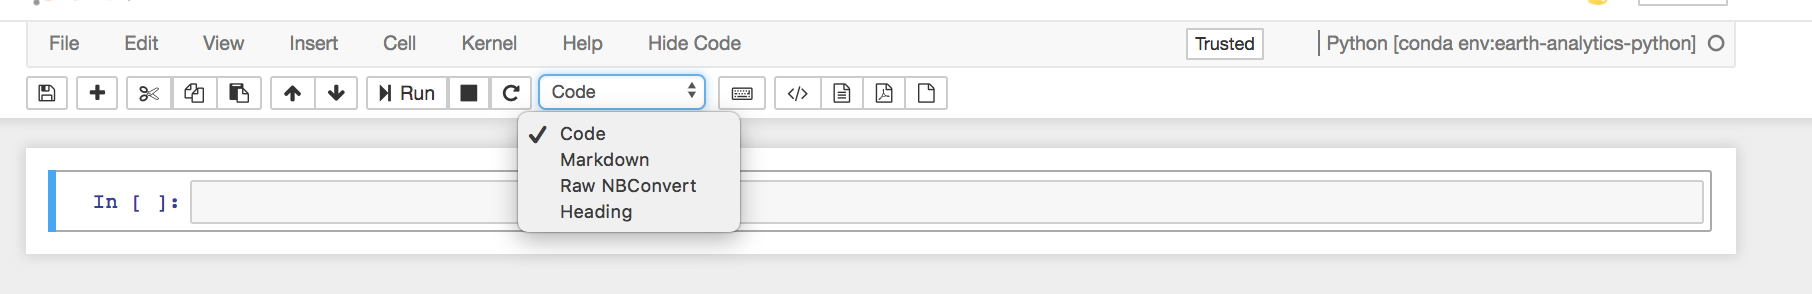
\includegraphics[scale=0.45]{Images/select-code-cell.png}
\caption{Você pode verificar o tipo de célula de qualquer célula em um Jupyter Notebook clicando na célula e olhando para o tipo de célula na toolbar.}\label{fig:JN-CodeCell}
\end{figure}
Os tipos mais utlizados são o {\tt Code} e o {\tt Markdown}. Deixemos a célula como tipo {\tt Code}, e façamos um primeiro código simples. Comecemos com o clássico dos clássicos da programação digitando {\tt print('Hello, World')}, como mostra a Fig. \ref{fig:JN-HelloWorld}. A execução do código nesta célula pode ser feita clicando no ícone de execução da célula na toolbar ou pressionando as teclas {\tt Shift + Enter}.
\begin{figure}[h]
\centering
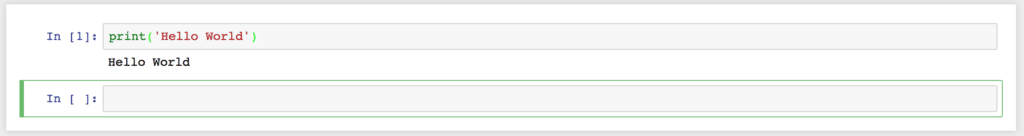
\includegraphics[scale=0.44]{Images/helloword.png}
\caption{Execução da célula de código muda {\tt In []} para {\tt In [1]}. O comando {\tt print} imprime o conteúdo entre parenteses, as aspas simples indicam que o conteúdo é do tipo texto. A saída da célula de código executada aparece logo abaixo da mesma.} \label{fig:JN-HelloWorld}
\end{figure}
O Jupyter Notebook oferece ajuda no próprio notebook para os commandos Python. Isso pode ser feito via os comandos:
\begin{enumerate}
    \item {\tt help()} mostra a documentação disponível para este objeto, método e função disponíveis para esse objeto.
    \item {\tt dir()} mostra as possíveis chamadas de objeto, método e função disponíveis para esse objeto.
\end{enumerate}
Teste por exemplo {\tt help(print)} e {\tt dir(print)}. Documentações mais detalhadas para comandos mais comuns podem ser encontradas no menu {\tt Help}. Além disso, sempre vale lembrar que existem uma farta documentação do Python e seus pacotes da internet.

O Jupyter Notebook também fornece alguns ``comandos mágicos'', que atalhos úties para vários problemas comuns na computação científica. Comandos mágicos vêm em dois tipos: ``magias de linha'', que são indicadas por um único prefixo \footnote{caso o Jupiter Notebook esteja com a opção Automagic ligada não é necessário o \% para usar ``mágicas de linha''.} \% e operam em uma única linha de entrada, e ``magias de célula'', que são indicadas por um prefixo \%\%  e operam em toda uma célula. Um exemplo é caso em queremos saber quanto tempo levamos para executar uma instrução. Para isso podemos usar o ``comando mágico'' {\tt timeit}, como no exemplo abaixo
\begin{lstlisting}[language=Python]
  %timeit list(range(100000))
\end{lstlisting}
essa instrução fará o Jupyter Notebook medir quanto tempo o sistema levará para construir uma lista de 100 mil elementos. Este comando também pode ser aplicado a toda uma célula como por exemplo:
\begin{lstlisting}[language=Python]
%%timeit
a = list(range(100000))
b = [n + 1 for n in a]
\end{lstlisting}
aqui medimos o tempo para se criar a lista {\tt a} e a lista {\tt b}. Em ambos os casos o tempo deve ser da ordem de alguns milisegundos (vai variar de computador para computador).
Uma lista com outros ``comandos mágicos'' pode ser acessada usando {\tt \%lsmagic}, referências mais detalhadas destes comandos podem ser obtidas usando {\tt \%quickref}. Veja e teste por exemplo os comandos {\tt \%hist}, {\tt \%ls}, {\tt \%magik}. Você aprenderá a usar essas ferramentas a medida que você for desenvolvendo mais e mais projetos no Python. Não se preocupe em memoriza-las. 


Um grande benefício do Jupyter Notebook é que ele permite combinar código (Code) e texto (Markdown) em um documento, para que você possa documentar facilmente suas ideias e fluxo de trabalho. Isso é extremamente útil para comunicar seu trabalho a outros físicos que poderão acompanhar mais detalhadamente sua ideiam mas também é útil para te orientar onde você parou em um projeto, mantendo registrada uma ideia que você estava seguindo. Lembre-se que para deixar a célula no tipo texto selecione a opção Markdown no menu da toolbar mostrado na Fig. \ref{fig:JN-CodeCell}. 

O Markdown é uma sintaxe legível por humanos (também conhecida como linguagem de marcação) para formatar documentos de texto. O Markdown pode ser usado para produzir documentos bem formatados, incluindo PDFs e páginas da web. Formatar um texto usando Markdown, é semelhante a usar as ferramentas de formatação em um editor de texto como o Microsoft Word ou o Google Docs. No entanto, em vez de usar ícones para aplicar a formatação, você usa uma sintaxe de comandos como {\tt **essa sintaxe coloca o texto em negrito no markdown**} ou {\tt \# Aqui está um título.} A Fig. \ref{fig:JN-Markdown-Raw} mostra um exemplo desta formatação. Uma célula Markdown é executada da mesma forma que uma célula de código. Após executarmos a célula com o código Markdown obtemos o texto formatado conforme as instruções. A saída do exemplo acima corresponde a Fig.
\ref{fig:JN-Markdown-Raw} esta mostrada na Fig. \ref{fig:JN-Markdown-prod}.
\begin{figure}[ht]
\centering
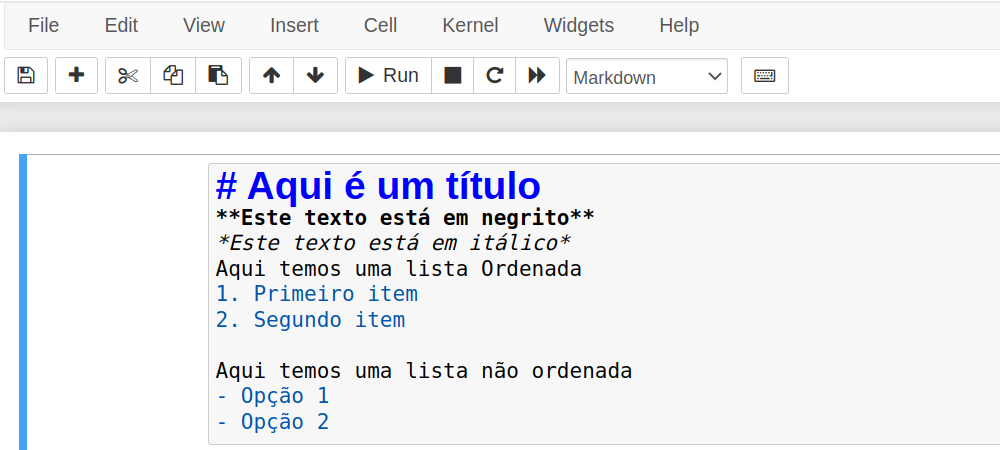
\includegraphics[scale=0.4]{Images/markdown-raw.png}
\caption{Uma célula Markdown com código antes de ser formatado. Nela vemos exemplos usuais de formatação para títulos, negrito, itálico e listas. Mais informações sobre sintaxe de formatação Markdown podem ser encontradas em \href{https://www.markdownguide.org/}{markdownguide.org}} \label{fig:JN-Markdown-Raw}
\end{figure}
\begin{figure}[h!]
\centering
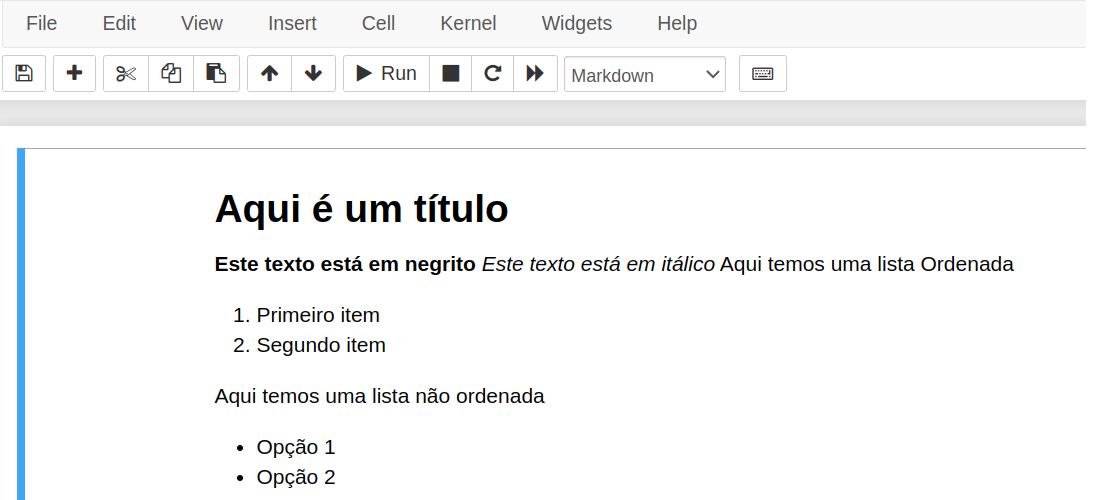
\includegraphics[scale=0.4]{Images/markdown-prod.png}
\caption{Saída de uma célula Markdown.} \label{fig:JN-Markdown-prod}
\end{figure}

O Markdown também é capaz de lidar com imagens, hyperlinks e vários outras necessidades de edição de texto. Para o trabalho em física é bastante importante que possamos escrever com facilidade expressões matemáticas. Isso é feito utilizando comandos \LaTeX. O \LaTeX é uma linguagem de preparação de documentos para composição tipográfica de alta qualidade. É mais frequentemente usado para documentos técnicos ou científicos de médio a grande porte, mas pode ser usado para quase qualquer forma de publicação. Este texto por exemplo foi preparado com \LaTeX, assim como o são a grande maioria das publicações científicas nas áreas de física. Você pode aprender mais sobre a linguagem \LaTeX no apêndice \ref{a:latex}. As Fig. \ref{fig:JN-Latex-in} e \ref{fig:JN-Latex-out} mostram respectivamente comandos \LaTeX em uma célula Markdown e mesma célula após o processamento.
\begin{figure}[h!]
\centering
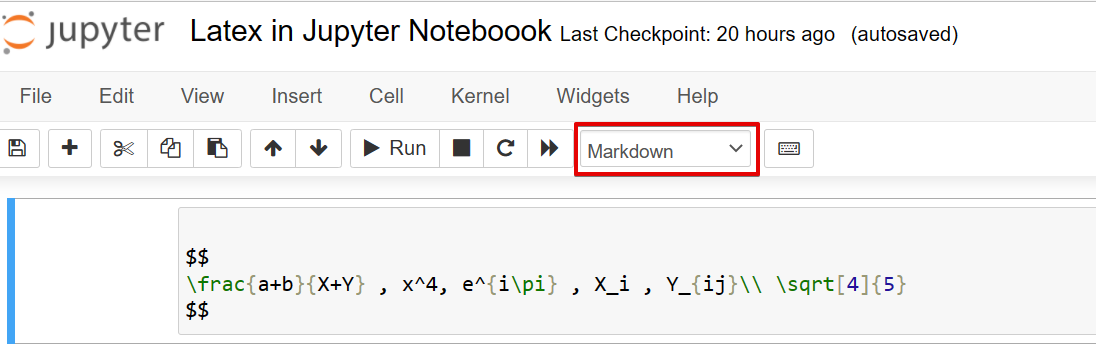
\includegraphics[scale=0.45]{Images/word-image-751.png}
\caption{Comandos \LaTeX em uma célula Markdown sendo utilizados para escrever uma equação.} \label{fig:JN-Latex-in}
\end{figure}
\begin{figure}[h!]
\centering
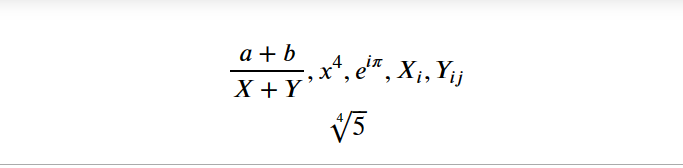
\includegraphics[scale=0.5]{Images/word-image-752.png}
\caption{Saída da célula Markdown da Figura anterior} \label{fig:JN-Latex-out}
\end{figure}

\section{Operações Matemáticas Simples}\label{sc:ops}

Até aqui, nosso conhecimento de Python nos permite fazer muito pouco, certamente nada que fosse útil para a física. A primeira coisa que precisamos conseguir utiliza-lo é entender como fazer operações aritméticas. Na maioria dos lugares onde você pode usar uma única variável em Python, você também pode use uma expressão matemática, como ``x+y''. Assim, por exemplo 
\begin{lstlisting}[language=Python]
  x = 1
  y = 2
  print(x+y)
\end{lstlisting}
computador calculará a soma de x e y para você e imprima o resultado. As operações matemáticas básicas são 
\[ \begin{array}{cc}
    x + y & \textrm{adição} \\
    x - y & \textrm{subtração} \\
    x * y & \textrm{multiplicação} \\
    x / y & \textrm{divisão} \\
    x ** y & x\text{ elevado a potência} y
\end{array} \]
Nesse ponto precisamos destacar que essas operações não agem somente em números e seu resultado depende do tipo de variáveis com as quais estamos lidando. Novamente, {\bf não entre em pânico}, vamos discutir rapidamente sobre variáveis na próxima seção e você ter mais informações no Apêndice \ref{ap:1.1}. Mas aqui vale um exemplo simples considere o caso:
\begin{lstlisting}[language=Python]
  x = 'Fi'
  y = 'si'
  z = 'ca'
  print(x+y+z)
  n = 3
  print(n*(x+y+z))
\end{lstlisting}
Nesse exemplo as variáveis x, y e z são do tipo {\it string} e o Python entende a operação $+$ como concatenação dessas strings. Já n é um variável do tipo inteiro e o Python entende a operação de multiplicar um inteiro com a string x+y+z, como concatenar n vezes essa string. Essa versatilidade do Python é uma de suas características úteis, mas também pode gerar erros.

Em Python, todos os operadores matemáticos $+$ (adição), $-$ (subtração), $*$ (multiplicação) funcionam como seria de esperar em números e variáveis numéricas. Ou seja contanto que você fique com os tipos de variáveis numéricas, adição, subtração e
multiplicação não deve haver muitos problemas. A divisão (/) tem algumas particularidades. Funciona perfeitamente em variáveis do tipo float, que são aquela usadas para descrever números via notação decimal, mas se operando entre inteiros: o resultado é sempre a parte inteira da resposta real. Veja por exemplo
\begin{lstlisting}[language=Python]
  print(1/2)
  print(1./2.)
  print(1./2)
\end{lstlisting}
No primeiro caso, ``1'' e ``2'' são ambos inteiros e o Python entende que resultado deve ser também um inteiro. No segundo caso ``1.'' e ``2.'' são ambos do tipo float e o Python entende que o resultado também deve ser do tipo float. O terceiro caso é um mix, ``1.'' é um float e ``2'' é um inteiro, o resultado será do tipo float.

O Python também possui dois outros tipos de ``divisão'' que são menos comuns que divisão usual, são elas:
\[ \begin{array}{cc}
    x // y & \textrm{O quotiente ou parte inteira da divisão} \\
    x \% y & \textrm{O resto ou operador módulo}
\end{array} \]
O quociente entre {\tt x} e {\tt y}, {\tt x//y},  é a parte inteira de {\tt x} dividida por {\tt y}, o que significa que {\tt x} é dividido por {\tt y} e a parte fracionária é descartada. O operador módulo entre {\tt x} e {\tt y}, {\tt x \% y}, é a parte inteira restante da divisão de {\tt x} por {\tt y}. Por exemplo, compare:
\begin{lstlisting}[language=Python]
  print(1.5 / 0.4)
  print(1.5 // 0.4)
  print(1.5 % 0.4)
\end{lstlisting}

As regras de precedência em Python são exatamente o que deveriam ser em qualquer
sistema matemático: (); então **; então *, /, \%, // na ordem da esquerda para a direita; e
finalmente +, - na ordem da esquerda para a direita.

Em Python o símbolo $=$ não significa 'é igual a', ou seja a expressão em Python {\tt x = y}, não é uma equação. No Python,  {\tt x = y} deve ser entendida como uma instrução para que o computador atribua a variável {\tt x} o valor da variável {\tt y}. O seguinte exemplo pode ser instrutivo
\begin{lstlisting}[language=Python]
  x = 1
  x = x + 1
  print('x =', x)
\end{lstlisting}
A primeira instrução atribui a variável {\tt x} o valor 1, a segunda instrução (que se entendida como uma equação matemática é absurda) pega o valor atual de {\tt x} é adiciona uma unidade. Quando a instrução {\tt print(x)} é executada imprimisse o valor de {\tt x} após a última instrução que o atualizou, ou seja obtemos {\tt x = 2}. Um truque  útil no Python, são as operadores {\it modificadores}, que permitem fazer alterações em uma variável da seguinte forma:
\[\begin{array}{cc}
{\tt x += y} & \text{\tt adicione\, y\, a\, x, ou seja, x = x + y}\\
{\tt x -= y} & \text{\tt subtrair y de x, ou seja x = x - y}\\
{\tt x *= y} & \text{\tt multiplicar x por y, ou seja x = x*y}\\
{\tt x /= y} & \text{\tt divide x por y, ou seja x = x/y}\\
{\tt x //= y} & \text{\tt divide x por y e arredonda para um inteiro, ou seja x = x//y}
\end{array}\]

Uma outra operação comum em Python é {\tt x == y}, esta é uma operação de comparação e seu resultado é uma variável do tipo {\it booleana}, ou seja é {\tt True} (verdadeiro) ou {\tt False} (falso). Ou seja a instrução {\tt x == y} é um condicional, i.e. equivale a pergunta ``o valor atual da variável {\tt x} é igual ao valor atual da variável {\tt y}?''. Algumas outras operações de comparação (e portando com saída True ou False) comuns no Python são
\[\begin{array}{cc}
{\tt x != y} & \text{\tt x é diferente de y?}\\
{\tt x < y} & \text{\tt x é menor que y?}\\
{\tt x <= y} & \text{\tt x é menor ou igual a y}\\
{\tt x > y} & \text{\tt x é maior que y?}\\
{\tt x >= y} & \text{\tt x é maior ou igual a y?}
\end{array}\]

\section{O ``Bê-a-bá'' sobre variáveis.}

Em programação, variáveis representam entre outras coisas instruções para computador guardar dados em sua memória, para serem usados posteriormente. São elementos fundamentais nos códigos computacionais. Por isso, vale a pena discutir como o Python lida com
variáveis. Tenha em mente que o que esta escrito no lado direito do operador de atribuição $=$ é um dado, equanto o que esta escrito no lado esquedo é um rótulo ou etiqueta para um local na memória do computador. Vamos ilustrar esse processo. Quando Python interpreta uma linha como {\tt x = 2} , ele começa do lado direito e segue a leitura para a esquerda. Então, dada a instrução {\tt x = 2} , o interpretador Python recebe o ``2'', reconhece-o como um inteiro e armazena-o em uma ``caixa'' de tamanho inteiro na memória. Em seguida, ele pega o rótulo {\tt x} e usa-o como um ponteiro para esse local de memória. Esse processo é mostrado na primeira parte da Fig. \ref{fig:memory}.
\begin{figure}[h]
\centering
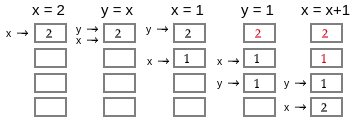
\includegraphics[scale=0.7]{Images/memory.png}
\caption{Atribuição de valores a variáveis e como o Python instruirá o computador a guardá-los na memória. Cada caixa representa uma localização na memória do computador.}\label{fig:memory}
\end{figure}

Quando encontra a instrução {\tt y = x}, o Python começa a partir da
direita {\tt x} e, reconhecendo x como um ponteiro para um local de memória, aponta o ponteiro {\tt y} para o mesmo local de memória. Esta é a segunda parte da Fig. \ref{fig:memory}. Continuando nesse processo, quando receber a instrução {\tt x = 1}, novamente o Python começa na direita e recebe o inteiro ``1'' e o aloca em uma `caixa'' de tamanho inteiro na memória. Só então ele executa o lado esquerdo da instrução, isso é, desloca o ponteiro rotulado como {\tt x} para esse novo espaço de memória. Isso não muda para onde o ponteiro {\tt y} esta apontado. Agora quando o Python receber a instrução {\tt y = 1}, ele ocupará um terceiro local na memória, e desviará o ponteiro {\tt y} para este local. Este local não será o mesmo para o qual esta apontado o ponteiro {\tt x}, para o Python não há razão para que os dois ponteiros apontem para o mesmo espaço de memória. Essa situação esta ilustrada na terceira parte da Fig. \ref{fig:memory}. Note que nesse momento não há nenhum ponteiro apontado para o bloco ocupado pelo valor $2$. Este bloco esta ocupado com dados que não são imediatamente apagados\footnote{É um ``lixo'' que fica na memória e pode comprometer o desempenho do sistema.}, mas o sistema entende que aquele espaço de memória esta livre para ser usado.

Essa interpretação de dados a direita e rótulos a esquerda permite que você faça algumas coisas muito úteis. Por exemplo, analisemos a instrução {\tt x = x + 1}. A direita o computador reconhecerá {\tt x} como um ponteiro apontando para uma valor, lê esse valor é o adiciona a $1$, como no final da Fig.\ref{fig:memory}, obtendo o valor $2$. Ele então desloca o ponteiro {\tt x} para aquela  nova ``caixa'' de memória.

Em Python também podemos atribuir múltiplos rótulos para um dado como por exemplo com a instrução {\tt w = x = y = z = 'Fisica'}. Neste caso, cada uma dessas variáveis
acabam apontando exatamente para o mesmo ponto na memória, até que sejam usadas para
outra coisa. O Python também permite que você atribua dados a mais de uma variável em uma mesma instrução. Por exemplo, {\tt a,b = 1, 2} funciona porque Python analisa os dados a direita da igualdade primeiro e reconhece um par de inteiro, então atribui esse par ao par de rótulos à esquerda. Isso é útil por nos permite trocar os valores de duas variáveis fazendo por exemplo {\tt x, y = y, x}. Analise por exemplo o código abaixo
\begin{lstlisting}[language=Python]
a = b = 1
a , b = b, a+b
print('a =', a, 'b=', b)
\end{lstlisting}
Para a maior parte das aplicações, conhecer detalhadamente como o Python gerencia variáveis não é necessário.

\subsection{Nomeando Variáveis}\label{sc:naming-var}
O nome de uma variável podem conter letras, números e o caractere \_. Esses nomes nunca podem começar com um número. E é importante lembrar que o Python diferencia maiúsculas e minúsculas. Ou seja portanto, {\tt Raio\_1} não é o mesmo que {\tt raio\_1}. É uma boa prática escolher nomes de variáveis que esclareçam a função daquela variável. Por exemplo, o nome {\tt m} é perfeitamente legal, mas quando um colega for ler o seu código o nome  {\tt massa\_partícula} é muito mais descritivo. O tempo extra que você gasta digitando esses nomes mais descritivos será mais do que compensado no momento em que você economiza depurando seu código!

As variáveis também não podem receber o mesmo nome de algumas palavras reservadas tais como:
\begin{table}[h!]
    \centering
    {\tt 
    \begin{tabular}{cccccc}
    and & as &  assert & async & await & break \\
    class & continue &  def & del & elif & else \\
    except & finally &  for & from & global & if \\
    import & in &  is & lambda & nonlocal & not \\
    or & pass & raise & return & try & while \\
    with & yield &  False & True & None &  \\
    \end{tabular}}
    \caption{Lista de Palavras Reservadas no Python 3}
    \label{tab:my_label}
\end{table}

É possível nomear uma variável usando o nome de uma função do Python (e.g. {\tt print}), mas a partir disso a função não ficará mais disponível. Portanto essa prática não é recomendável. Você também deve evitar nomes como ``I'', ``l'', ``O'' e ``o'' para evitar confusão com os números 1 e 0. Nomes como {\tt n,i,j,k} são usualmente reservados para contadores inteiros. Essas e muitas outras regras e convenções estão codificadas em um guia de estilo chamado PEP8 que faz parte da documentação do Python, e pode ser acessado em \href{https://peps.python.org/pep-0008/}{https://peps.python.org/pep-0008/}.

\subsection{Alguns tipos de variáveis}

Todas as variáveis em Python possuem uma certa natureza ou como se diz são de certos tipos. Isso significa que os dados que elas rotulam têm certas propriedades que ditam como elas são usadas. Tipos diferentes têm propriedades diferentes e são utilizados para diferentes aplicações. Você sempre pode determinar o tipo de uma variável (ou de um dado) usando a função interna {\tt type()}. Veja o exemplo abaixo:
\begin{lstlisting}[language=Python]
dimensao = 3
FortyTwo = 'Vida, Universo e Tudo Mais'
pi = 3.1415
z = 1 + 1j
Fibonacci_5 = [1, 1, 2, 3, 5]
type(dimensao),type(FortyTwo),type(pi),type(z),type(Fibonacci_5)
\end{lstlisting}

Existem diversos tipos diferentes de variáveis em Python. Os dois tipos mais comuns 
podem ser divididos em {\it tipos numéricos} e {\it tipos sequenciais}. Tipos numéricos
contêm dados que representam um números únicos, como por exemplo ``42'', ``3,1415'' e ``1 + 3i11. Tipos sequenciais contêm dados com vários objetos, que podem ser números ou
caracteres, ou mesmo coleções de diferentes tipos de objetos. Um dos pontos fortes do Python é que ele automaticamente converte entre tipos de variáveis conforme é necessário e se possível. Essa mutabilidade das variáveis também pode levar a armadilhas que produzem erros no código. Discutiremos aqui os tipos numéricos e sequenciais, você pode ver mais sobre outros tipos no apêndice \ref{ap:1.1}.

\subsubsection{Tipos Numéricos}
As variáveis numéricas em Python, podem ser de 3 tipos: inteiros (type: int ), números de ponto flutuante (type: float) e números complexos (type: complex).

\paragraph{Integer:} O inteiro é o tipo numérico mais simples em Python. Os inteiros são
usados para contar itens ou acompanhar quantas vezes você fez alguma coisa. Eles podem ser negativos ou positivos, ou seja eles correspondem ao que chamamos de números inteiros. Lembre que como já discutimos na seção \ref{sc:ops}, variáveis do tipo {\tt int} não se dividem como esperado: Em Python, {\tt 1/2} resulta em {\tt 0}, porque $2$ cabe em $1$ zero vezes.
\paragraph{Float:} O tipo “floating point” (i.e. ponto flutuante) é um número que contém um ponto decimal dividindo sua parte inteira de sua parte fracionária. Por exemplo, $3.1415$ e $9.81$ são do tipo float. Tipos float também podem ser escritos usando notação científica por exemplo {\tt 6.022e23} corresponde a $6.022 \times 10^23$ é um float. 
\paragraph{Complex:} Números complexos são embutidos no Python, que usa $j=\sqrt{-1}$ para unidade imaginária. Essas variáveis são do tipo $a+bj$, onde a parte real do número é $a$ e a parte imaginária é $b$. O Python executa corretamente as operações elementares com números complexos.

Números em Python N são objetos (na verdade, tudo em Python é um objeto) e têm certos
{\it atributos}, acessados usando a notação: {\tt <objeto>.<atributo>} (este uso do
período não tem nada a ver com o ponto decimal que aparece em um tipo float. Alguns atributos são valores simples: por exemplo, objetos de números complexos têm a
atributos real e imag , que são as partes real e imaginária (ponto flutuante) do
número. Teste por exemplo
\begin{lstlisting}[language=Python]
(1 + 2j).real
(1 + 2j).imag
\end{lstlisting}
Nesses objetos também é possível aplicar neles {\it métodos}, ou seja aplicar algumas funções no mesmo. Por exemplo
\begin{lstlisting}[language=Python]
(1 + 2j).conjugate()
42.bit_length
(3.14159265359).bit_length
\end{lstlisting}
Digitando-se {\tt <objeto>.} e pressionando a telca Tab o Jupyter Notebook abrirá um menu com uma lista de métodos que são possíveis de se aplicar naquele objeto. 

\subsubsection{Tipos Sequenciais}
Tipos sequenciais são coleções de itens que são rotulados por um nome de variável. Os itens individuais dentro da coleção são separados por vírgulas, e referido por um índice entre colchetes após o nome da variável. Veja o exemplo:
\begin{lstlisting}[language=Python]
Disciplinas  = ('Termodinamica', 'Eletromagnetismo', 
        'Quantica', 'Estado Solido')
print(Disciplinas[2])
\end{lstlisting}
O resultado destas instruções deve ser {\tt Quantica}. Note que o índice começa a contar de 0. Você pode usar também índices negativos para contar de trás para a frente, por exemplo
\begin{lstlisting}[language=Python]
print(Disciplinas[-1],Disciplinas[-3])
\end{lstlisting}
Vamos examinar agora alguns tipos sequencias específicos utilizados no Python.

\paragraph{Tuple} As Tuplas são indicadas por parênteses: (). Itens em tuplas podem ser
qualquer outro tipo de dados, incluindo outras tuplas. Tuplas são {\it imutáveis},
o que significa que uma vez definidos seus conteúdos não podem ser alterados. Por exemplo, as instruções abaixo irão gerar um erro:
\begin{lstlisting}[language=Python]
teste = (1,2,3)
type(a)
print(a[1])
a[1] = 'dois'
print(a)
\end{lstlisting}

\paragraph{List} As listas são indicadas por colchetes: [ ]. As listas são praticamente o
iguais às tuplas, mas são {\it mutáveis}: itens individuais em uma lista podem ser
modificados. As listas podem conter qualquer outro tipo de dados, incluindo outras listas. Note a diferença trocando os parênteses por colchetes na primeira linha das instruções acima
\begin{lstlisting}[language=Python]
teste = [1,2,3]
type(a)
print(a[1])
a[1] = 'dois'
print(a)
\end{lstlisting}

\paragraph{String} Uma string é uma sequência de caracteres. As strings são delimitadas por
aspas simples ou duplas: " " ou ' '. Strings são {\it imutáveis}, como tuplas. Ao contrário das listas ou tuplas, as strings só podem incluir caracteres. O exemplo abaixo mostra algumas operações com strings.
\begin{lstlisting}[language=Python]
Palavra='trabalho e Energia'
print(Palavra)
print(Palavra[1])
print(Palavra[:5])
print(Palavra[-4:])
print(Palavra.capitalize())
print(Palavra.count('a'))
print(Palavra.split())
\end{lstlisting}

\paragraph{Dictionary} Os dicionários são indicados por colchetes: { }. Eles são dif-
diferente dos outros tipos sequenciais em Python, pois em vez de índices numéricos que eles usam keywords são rótulos de strings.

\paragraph{Range} Um tipo range representa uma sequência {\it imutável} de números e é comumente usado para fazer um loop de um número específico de vezes em loops. Um range é criado por uma instrução {\tt range({\it start}, {\it stop}, {\it step})}, onde {\it start} é o índice inicial\footnote{O argumento {\it start} é opcional, se omitido o range começa por padrão em 0.}, {\it stop} o índice final (que não é incluído), e {\it step}\footnote{O argumento {\it step} é opcional, se não incluído o intervalo padrão é 1.}  o intervalo entre os índices. Veja o exemplo abaixo
\begin{lstlisting}[language=Python]
Pares = range(0,100,2)
print('Pares =', type(Pares))
print(Pares)
print('Os primeiros pares:', Pares[0], Pares[1], Pares[2])
Pares_list = list(Pares)
print(Pares_list)
\end{lstlisting}
A última instrução mostra como converter uma variável tipo range em uma variável tipo list.

Conforme mencionado acima na descrição das listas, uma lista pode conter como elementos outras listas. Uma lista de listas lembra bastante uma matriz bidimensional. Veja por exemplo:
\begin{lstlisting}[language=Python]
matrix = [[1,2,3],[4,5,6]]
print(matrix[1][1])
\end{lstlisting}
Que resulta em 5 (não se esqueça que os índices começam em 0). Há alguma utilidade em visualizar listas desse tipo como matrizes, mas estes objetos não operam como matrizes. Teste por exemplo {\tt print(matrix + matrix)} e você verá que o Python apenas concatena as listas. Novamente, {\bf não entre em pânico}, algumas bibliotecas como o SciPy e o NumPy vão adicionar funcionalidades que nos permitirão usar matrizes como conhecemos.

Listas são objetos bastante úteis e comuns. Veja o exemplo abaixo para algumas operações úteis com listas.
\begin{lstlisting}[language=Python]
primes = [2, 3, 5, 7, 11, 13]
primes.append(17)
print(primes)
primes.reverse()
print(primes)
primes.pop(6)
print(primes)
primes.sort()
print(primes)
primes = primes+2*['a']+['b']+['c']+['b']
print(primes)
primes.remove('a')
print(primes)
primes.pop(-1)
print(primes)
\end{lstlisting}

A tabela abaixo mostra os métodos disponíveis para operar em listas:
\begin{table}[h!]
    \centering
    \begin{tabular}{l l}
    {\tt append({\it element})}     & Anexa {\it element} ao final da lista  \\
    {\tt extend({\it other\_list})}     &  Estende a lista com os elementos de {\it other\_list}\\
    {\tt index({\it element})} & Retorna o índice mais baixo da lista que contém {\it element} \\
    {\tt insert({\it index, element})} & Insere {\it element} no índice {\it index} \\
    {\tt pop({\it index})} & Remove o elemento de índice {\it index}+1\\
    {\tt reverse()} & Reverte a ordem da lista\\
    {\tt remove({\it element})} & Remove a primeira ocorrência de {\it element}\\
    {\tt sort()} & Ordena a list\\
    {\tt count({\it element})} & Conta o número de ocorrências de {\it element}
    \end{tabular}
    \caption{Alguns métodos disponíveis para operar em listas.}
    \label{tb:list-methods}
\end{table}

\section{Instruções de Controle}

Poucos programas de computador são executados de forma puramente sequencial, uma instrução após outra na sequência escrito no código-fonte. É comum que durante a execução do programa, dados sejam inspecionados e blocos de código executados a depender de
algum teste realizado nestes dados. Instruções de controle são instruções que permitem que um programa siga caminhos diferentes dependendo de algum evento. Essas instruções fazem o papel análogo a instruções da vida real do tipo “Se você está com fome, coma.” ou ainda “Enquanto a luz estiver vermelha, não entre.”  Todas essas instruções têm a mesma estrutura básica: (a) a própria instrução: ``se'' ou ``Enquanto'', (b) um  ``condicional'', que é uma afirmação que deve ser avaliada como verdadeira (True) ou falsa (True): ``você está com fome'' ou ``A luz está vermelha''. E há a ação a ser executa: ``coma'' ou ``não entre''. 

Nessa seção, discutiremos 3 instruções de controle do Python, são elas:\\ 
\begin{center}
    {\tt if ... elif ... else}, {\tt while} e {\tt for}.
\end{center}
Antes de explorarmos como essas instruções funcionam vamos entender um pouco mais sobre condicionais.

\subsection{Condicionais}

Um condicional é qualquer coisa que o Python possa avaliadar como  True (verdadeiro) ou falso. Geralmente um condicional será uma expressão de uma relação entre dados que são comparados usando operadores de comparação como {\tt ==, !=, <, <=, >, >=} . Veja os seguintes exemplos:
\begin{lstlisting}[language=Python]
print(1<2)
print('a' in 'Fisica')
print('b' not in 'Fisica')
print(22/7 < 3.14)
print(10**2 == 100.)
print([1,2,3] != [1,2,'tres'])
\end{lstlisting}
Condicionais podem também ser combinados usando operadores booleanos {\tt and, or} e {\tt not}. Operadores booleanos tem a menor ordem de precedência em todo o Python. A tabela abaixo mostra como esses operadores booleanos agem
\begin{table}[h!]
\begin{minipage}{.36\textwidth}
    \centering
    {\tt 
    \begin{tabular}{c c c c}
     True & and & True & -> True\\
     True & and & False & -> False \\
     False & and & True & -> False \\
     False & and & False & -> False
    \end{tabular}}
    \end{minipage}
    \begin{minipage}{.36\textwidth}
    \centering
    {\tt 
    \begin{tabular}{c c c c}
     True & or & True & -> True\\
     True & or & False & -> True \\
     False & or & True & -> True \\
     False & or & False & -> False
    \end{tabular}}
    \end{minipage}
    \begin{minipage}{.3\textwidth}
    \centering
    {\tt 
    \begin{tabular}{c c c c}
      & not & True & -> False\\
      & not & False & -> True \\
     \end{tabular}}
    \end{minipage}
    \caption{Algebra Booleana}
    \label{tab:boolean}
\end{table}

\subsection{if ... elif ... else}

A instrução de controle mais básica em Python\footnote{ou qualquer outra linguagem de computador}, é a instrução equivalente ao ``se''. Ele permite que você diga ao computador o que fazer se alguma condição é satisfeita. A sintaxe é a seguinte:
\begin{lstlisting}[language=Python]
if <condicional 1>:
    <instrucao 1>
    <instrucao 2>
    ...
elif <condicional 2>:
    <instrucao 3>
    <instrucao 4>
    ...
else:
    <instrucao 5>
\end{lstlisting}
Observe a indentação do código, i.e. os espaços em branco (um Tab) entre {\tt if ... elif ... else}. Em Python, esses espaços em branco definem que o grupo de comandos deve ser executado caso o condicional seja True. Ou seja a indentação não é opcional. A identação serve para informar ao Python, qual bloco de instruções é deve ser executado se aquele condicional for verdadeiro. As instruções {\tt elif} (ou se) e {\tt else} (``ou então'') estendem a instrução {\tt if}. A instrução {\tt elif}, é uma abreviação para “else if” adiciona outro {\tt if} que é testado se e somente se o primeiro condicional for falso. Você pode utilizar quantos {\tt elif} forem necessários, os condicionais serão testados na ordem em que aparecerem. A instrução {\tt else}, é executada  se nenhuma das instruções {\tt elif} anteriores, ou a inicial {\tt if}, for verdadeira.

{\bf Exemplo:} No calendário gregoriano, um ano é bissexto se for divisível por 4 com a exceção de que os anos divisíveis por 100 não são bissextos, a menos que também sejam
divisíveis por 400. O programa Python a seguir determina se ano é bissexto.
\begin{lstlisting}[language=Python, frame=lines,basicstyle=\footnotesize, caption={Determinando se um ano é bissexto.}, label={lst:bissexto}]
ano = int(input('Qual o ano?')

if not ano % 400:
    is_leap_year = True
elif not year % 100:
    is_leap_year = False
elif not year % 4:
    is_leap_year = True
else:
    is_leap_year = False
print('O ano ', year, ' e bissexto')
\end{lstlisting}

\subsection{while}

A instrução while é usada para repetir um bloco de comandos até que uma condição
deixe de ser satisfeita. Considere o exemplo abaixo:
\begin{lstlisting}[language=Python]
i = 0
while i < 10:
    i += 1
    print(i, end=',')
print('fim')
\end{lstlisting}
Cada vez que o bloco de instruções do {\tt while} é executado, o contador $i$ (que começa em 0), é acrescido de 1 e seu valor é impresso. Esse bloco será executado até que $i$ tenha o valor $10$, quando o Python sai do loop e executa o comando {\tt print(fim}).

Podemos combinar loops {\tt while} com {\tt if ... elif...else} para obtermos decisões mais complexas. Veja o exemplo a seguir
{\bf Exemplo:} Em 1937, o matemático alemão Lothar Collatz, propôs a seguinte sequência de inteiros positivos: O primeiro termos da sequência é $c_1 =n$, onde $n$ é um número inteiro positivo. Dado o $c_k$, o $k$-ésimo termo da sequência, o termo seguinte é obtido fazendo
\[a_{k+1} =\left\{\begin{array}{cl} a_k/2 & \textrm{se } a_k\textrm{ é par}\\
3a_k+1 & \textrm{se } a_k \textrm{ é ímpar}
\end{array}\right.\]
Collatz conjecturou que qualquer que seja o inteiro inicial $c_1$ a sequência sempre termina em $1$. Até o momento em que escrevo essas notas (2022), a Conjectura de Collatz nunca havia sido provada, permanecendo como um problema em aberto (para mais detalhes veja a Ref. \cite{collatzconjecture}. 

Nesse exemplo, iremos obter a sequência de Collatz para um inteiro positivo qualquer. Tente resolver antes de checar uma possível solução abaixo.

\begin{lstlisting}[language=Python, frame=lines,basicstyle=\footnotesize, caption={Testando a conjectura de Collatz}, label={lst:Collatz}]
num = int(input('Qual o inteiro positivo inicial?'))
print('A sequencia de Collatz para', num)
while num != 1:
    if num % 2 == 0:
        num = int(num/2)
        print(num, end=',')
    else:
        num = int(3*num+1)
        print(num, end=',')
\end{lstlisting}

Loops {\tt while} podem ser estendidos usando alguma palavras chave:

\paragraph{continue} A instrução {\tt continue} move a execução do programa para o topo
o bloco {\tt while} sem terminar a parte do bloco seguinte a instrução continue.

\paragraph{break} A instrução {\tt break} interrompe a execução do loop e recomeça o código diretamente para a linha seguinte ao bloco {\tt while}. Em outras palavras, ele ``sai'' do loop.

\paragraph{else} Um comando {\tt else} no final de um bloco {\tt while} é usado para delinear um bloco de código que é executado depois que o bloco {\tt while} termina, mas
o código neste bloco não é executado se o bloco {\tt while} for encerrado via
um comando de pausa.

O exemplo a seguir deve esclarecer o uso dessas instruções.

{\bf Exemplo:} Você precisa escrever um programa que teste se um número é
prima ou não. O programa deve pedir o inteiro para testar, em seguida, imprima uma mensagem informando o primeiro fator encontrado ou informando que o número é primo. Tente você mesmo antes de examinar o exemplo abaixo:

\begin{lstlisting}[language=Python, frame=lines,basicstyle=\footnotesize, caption={Testando se um número é primo}, label={lst:isprime}]
Number = int(input('Qual inteiro iremos testar?'))
TestNumber = 2
while TestNumber < Number :
    if Number % TestNumber == 0 :
        print(Number , 'e divisivel por' , TestNumber , end='.')
        break
    else:
        TestNumber += 1
else:
    print(Number , 'e primo', end ='.')
\end{lstlisting}
Esta não é a forma mais eficiente de determinar se um número inteiro muito grande é primo.

\subsection{for}
O loop {\tt for} itera sobre os itens em uma sequência, repetindo o bloco de loop uma vez
por item. A sintaxe mais básica é a seguinte:
\begin{lstlisting}[language=Python]
for <iterador> in <tipo sequencial>
    <instrucao 1>
    <instrucao 2>
    ...
\end{lstlisting}
Cada vez que passar pelo loop, o valor do {\tt iterador} será o valor do
próximo elemento em {\tt <tipo sequencial>} . Vejamos o exemplo abaixo, 
\begin{lstlisting}[language=Python]
lista = [1,'a',[1,2]]
index = 0
for t in lista:
    print('o elemento', index, '=', t)
    index += 1
\end{lstlisting}
o código imprime cada um dos elementos de {\tt lista}.
Você pode usar qualquer tipo sequencial, mas tipos imutáveis são preferíveis para se evitar alterar a sequência que esta controlando o loop. Por exemplo, o exemplo abaixo vai gerar um loop infinito:
\begin{lstlisting}[language=Python]
lista = [1,'a',[1,2]]
index = 0
for t in lista:
    print('o elemento', index, '=', t)
    lista += index*[t]
    index += 1
\end{lstlisting}

O exemplo abaixo mostra como podemos usar uma string para controlar o {\tt for}.
\begin{lstlisting}[language=Python]
letras = 0
for t in 'Palavra':
    letras +=1
\end{lstlisting}
No cálculos numéricos, é mais comum usar o comando for sobre um intervalo numérico gerado com {\tt range}
\begin{lstlisting}[language=Python]
N, S = 100, 0
for t in range(0,N,1):
    S += t 
print(S)    
\end{lstlisting}

O exemplo abaixo mostra como gerar a sequência de Fibonacci e aproximar a razão áurea.
\begin{lstlisting}[language=Python, frame=lines,basicstyle=\footnotesize, caption={Sequência de Fibonacci e a Razão Áurea }, label={lst:fibonacci}]
N = 100
fibonacci = [1, 1]

type(fibonacci)
for n in range(2,N):
    fibonacci.append(fibonacci[n-1]+fibonacci[n-2])
print(fibonacci)
print('Razao Aurea aproximadamente', fibonacci[n]/fibonacci[n-1])
\end{lstlisting}

A instrução {\tt for} também permite o uso das mesmas palavras-chave usadas para {\tt while}. Além, disso o Python fornece uma sintaxe muito útil e concisa para criar e manipular tipos sequenciais. Quando aplicada a listas essa sintaxe é chamada de {\it List Comprehensions}. A ideia é usar instruções {\tt for} e {\tt if} no interior da indicação de uma lista. A sintaxe é
\begin{lstlisting}[language=Python]
lista_1 = [ <expressao> for <iterador> in <tipo sequencial]
lista_2 = [<expressao> if <condicional> else <expressao> 
        for <iterador> in <tipo sequencial>]
\end{lstlisting}

O uso de {\it List Comprehensions} deve ficar mais claro nos exemplos abaixo:

{\bf Exemplo:} Suponha que você tenha uma lista de medidas de comprimento feitas em polegadas. Precisamos converter essas medidas para centímetros (1 polegada = 2.54 cm).
\begin{lstlisting}[language=Python]
lista_de_medidas = [1.1, 1.3, 1.75, 2.1, 9.1, 10.2, 9.8 ]
medidas_cm = [2.54*medida for medida in lista_de_medidas]
\end{lstlisting}

{\bf Exemplo:} Crie uma lista com os números entre 0 e 100 que são divisíveis por 6, mas não são divisíveis por 5.
\begin{lstlisting}[language=Python]
max = 100//6
numeros=[6*n for n in range(max) if (not 6*n % 5 ==0)]
print(numeros)
\end{lstlisting}

\section{Funções}

Uma função é um bloco de código que recebe seu próprio nome para que possa ser
usado repetidamente por várias partes de um programa. Nesse sentido uma função pode ser um código para realizar um cálculo matemático, ou um código para fazer algo, como desenhar um gráfico ou salvar uma lista de números. No Python, a primeira linha de uma função é definida com a palavra-chave {\tt def} (vem de {\it definition}) seguido pelo nome da função, a lista de argumentos e dois pontos(:). As demais linhas contém as operações que compõem a função, que ficam em um bloco de código indentado. Lembre que no Python, a indentação funciona como um organizador para que o Python saiba a qual parte do código aquele bloco pertence. A sintaxe basica de uma função é a seguinte
\begin{lstlisting}[language=Python]
def <nome>(<argumentos>):
    <codigo da funcao>
\end{lstlisting}
O {\tt<nome>} estabelece o nome pelo qual a função será chamada. As mesmas regras para se nomear uma variável (ver \ref{sc:naming-var}, valem para nomear funções. As funções no Python, podem possuir argumentos, de forma análoga a suas análogas em matemática.  Esses argumentos são uma lista de coisas que a função precisa para fazer seu trabalho. Os argumentos vem dentro de parênteses imediatamente após o nome da função. O código indentado será executado sempre que a função for chamada e usará os argumentos dados entre parênteses como parâmetros.
As funções também podem retornar valores usando a palavra-chave {\tt return} seguida por uma expressão  a ser devolvida. Neste caso a syntaxe é
\begin{lstlisting}[language=Python]
def <nome>(<argumentos>):
    <codigo da funcao>
    return <retorno1>, <retorno2>, ..., <retorno3>
\end{lstlisting}

{\bf Exemplo:} Vamos escrever uma função que soma os dígitos de um número. Tente você antes
de ver o exemplo abaixo.
\begin{lstlisting}[language=Python]
def soma_digitos(n):
    n_name = str(n)
    s = 0
    for i in n_name:
        s += int(i)  
    return s
\end{lstlisting}

A função também pode retornar múltiplos valores. Vejo o exemplo

\begin{lstlisting}[language=Python]
def energia_momento(m,v):
    K = (1/2)*m*v**2
    p = m * v
    return K, p
\end{lstlisting}

Em várias situações é interessante definir argumentos com valores padrão. Em Python, eles são conhecidos como argumentos de palavras-chave, e nesse caso apontar o valor dos argumentos passa a ser opcional, i.e. a função usa o argumento padrão quando um novo valor não é usado. Quando os argumento são passados com palavras-chave, eles podem ser chamados em qualquer ordem. Os argumentos de palavra-chave são definidos pelo nome do argumento (a palavrachave), um sinal de igual ( = ), e o valor padrão que é usado se o argumento não for fornecido quando a função é chamada. A sintaxe básica é a seguinte
\begin{lstlisting}[language=Python]
def <name>s(<key word1> = <val1>, ..., <key wordn> = <valn>):
    <codigo da fucao>
\end{lstlisting}




\section{Bibliotecas: o Básico}


Construção de um barra de progresso para algorítimos que levem tempo

\begin{lstlisting}[language=Python]
rom tqdm.notebook import tqdm
from time import sleep

for i in tqdm(range(10)):
    sleep(3)
\end{lstlisting}

\section{Gráficos Simples}

\section{Lendo dados de arquivos}

\section{Exercícios}
\begin{enumerate}
    \item Comente com $\#$ os códigos dados como exemplo nesse capítulo, indicado o que cada linha ou bloco instrui o computador a fazer.
    \item Escreva um programa que pede para o usuário escrever um número inteiro entre $0$ e um milhão, e então escreve esse número por extenso.
    \item  Quando escrevemos um número $n$ na base decimal estamos implicitamente dizendo:
\[ n = d_N 10^N + d_{N-1} 10^{N-1} + \cdots + d_2 10^2 + d_1 10^1 + d_0 10^0 \]
onde $N+1$ é o número de dígitos de $n$ e $d_k = 0,\cdots,9$, $k=0,\cdots,N$ são os dígitos desse número ($d_N \neq 0)$. Da mesma forma $n$ pode ser escrito na base binária, onde os digitos dão $b_j = 0,1 $ fazendo
\[ n = b_m 2^m + b_{m-1} 2^{m-1}+ \cdots + b_2 2^2 + b_1 2^1 + b_0 2^0. \]
É claro que o maior número que pode ser escrito em base binária com $m$ dígitos é
\[ n_{max} = 2^m + 2^{m-1}+ \cdots + 2^2 + 2^1 +  2^0 = 2^{m+1}-1 \]
resultado que obtemos reconhecendo a série geométrica finita na expressão acima. Vamos escrever um código que converte um número da base decimal para a base binária.
    \item Um problema clássico em olimpíadas de matemática para o nível fundamental é o {\it Problema dos Armários}. O problema é o seguinte: Em uma escola existem 1000 armários numerados (de 1 a 1000) e 1000 alunos. No primeiro dia de aula, o Diretor reúne todos os 1000 alunos em fila. O Diretor então manda que o primeiro aluno da fila abra todos os armários. Após esse aluno terminar a tarefa, o diretor ordena que o próximo estudante (i.e. o segundo aluno da fila) feche todos os armários com número par. Quando ele conclui a tarefa o diretor, manda que o terceiro aluno da fila mude o estado de todos os armários com número divisível por 3. Mudar o estado significa se o armário estiver aberto, ele irá fecha-lo e se o armário estiver fechado, ele irá abri-lo. Ao quarto aluno, o diretor mandará que mude o estado de todos os armários divisíveis por 4, ao quinto aluno que mude o estado de todos os armários divisíveis por 5, e assim sucessivamente até que todos os 1000 alunos tenham participado.
    \begin{enumerate}
        \item Escreva um programa para simular o problema descrito. O programa deve ser capaz de determinar aos final do processo: quais armários estão abertos, quais estão fechados e o número total de armários abertos.
        \item Como disse na introdução este é um problema de matemática. A resolução esperada do {\it Problema dos Armários} não envolve computação, mas sim a compreensão de propriedades de divisores de números inteiros. Vamos tentar entender essa propriedade usando um programa de computador: Construa um programa que analisa os 10 mil primeiros números inteiros e separa em uma lista aqueles que tem um número ímpar de divisores. Verifique que todos estes números são quadrados perfeitos. Suponha que esta é uma propriedade geral, como ela pode ser usada para responder o {\it Problema dos Armários}.
        \item {\bf (Opcional)} Demonstre matemáticamente a propriedade conjecturada no item anterior, i.e.  ``Um núemero inteiro positivo é um quadrado perfeito se e somente se ele possui um número ímpar de divisores''.
    \end{enumerate}
    \item Escreva uma função que calcule o fatorial de um número inteiro.
\end{enumerate}

